\documentclass{article}
\usepackage[utf8]{inputenc}
\usepackage[spanish]{babel}
\usepackage{graphicx}
\usepackage{verbatim}
\usepackage{moreverb}
\usepackage{amsmath}
\usepackage{amsfonts}
\usepackage{amssymb}
\usepackage{fancybox}
\usepackage{float}
\usepackage{fancyvrb}
\usepackage{color}
\usepackage{hyperref}
\usepackage{multirow}
\usepackage{subfigure}


\usepackage{anysize}
\marginsize{1.5cm}{1.5cm}{1cm}{1cm}

\renewcommand{\shorthandsspanish}{}

\newcommand{\HRule}{\rule{\linewidth}{0.5mm}}

\begin{document}

\thispagestyle{empty}

%%%%%%%%%%%%%%%%%%%%%%%%%%%%%%%%% PORTADA %%%%%%%%%%%%%%%%%%%%%%%%%%%%%%%%%%%%%%

\begin{titlepage}
\begin{center}

%Espacio antes del logo del itba
\Large \  \\[1.5cm]


\includegraphics[scale=0.40]{Imagenes/logo_itba}\\[1cm]
\textsc{\LARGE Criptografía y Seguridad}\\[1.5cm]
\textsc{\Large Trabajo práctico $\text{N}^{\circ}$2}\\[0.5cm]

\HRule \\[0.4cm]
{ \huge \bfseries Secreto Compartido en Imágenes con Esteganografía}\\[0.4cm]
\HRule \\[1.5cm]

\Large Autores: \\ [0.25cm]
\begin{tabular}{l @{\ \ -\ \ }l}
\Large Pablo Ballesty & \Large 49359\\[0.2cm]
\Large Nicolás Magni & \Large 48008\\[0.2cm]
\end{tabular}



\vspace{1cm}

\vfill
% La fecha queda abajo.
{\large \today}

\end{center}
\end{titlepage}

%%%%%%%%%%%%%%%%%%%%%%%%%%%%%%%%%%%%%%%%%%%%%%%%%%%%%%%%%%%%%%%%%%%%%%%%%%%%%%%%

\tableofcontents
\clearpage

\abstract{

El objetivo del presente informe es detallar las deciones tomadas durante el diseño y la implementación del Trabajo Práctico.
Así también, se presentan los resultados obtenidos a partir de las imágenes que envió la cátedra y se realiza un análisis de
los mismos. Se detallan las dificultades encontradas, y las soluciones propuestas. También se presentan conclusiones y posibles
extensiones del algoritmo.

}

\section{Introducción}

El Trabajo Práctico consiste en la implementación de un algoritmo de secreto compartido, aplicado a imágenes. Los algoritmos
de secreto compartido, consisten en ocultar información sensible, la cual llamaremos \emph{el secreto}, utilizando $n$ claves, de las cuales, para la
recuperación del secreto, serán necesarias $k$ (con $k \le n$).\\

Como en este caso, las claves son imágenes, al momento de generar las mismas, se utiliza una técnica de \emph{esteganografía} con el fin
de que el ojo humano no note que se trata de claves.\\

El algoritmo que se implementa en el trabajo se extrajo de la publicación \textbf{\emph{``Improvements in Geometry-Based Secret Image Sharing Approach
with Steganography``}} realizada por \textbf{Mustafá Ulutas}, \textbf{Vasif V. Nabiyev} y \textbf{Guzin Ulutas}, de la Universidad de Karadeniz, Turquía.

\section{Desarrollo}

El algoritmo no resulta difícil de implementar, sin embargo, require de tener especial cuidado en ciertos aspectos, para obtener resultados 
exitosos. A continuación, se detallan las dificultades que presenta el algoritmo, y como éstas fueron resueltas en la práctica.

\subsection{Algoritmo de distribución}

El algoritmo de distribución consiste, en dadas $n$ imágenes (las cuales llamamos \emph{imágenes cover}), una imágen secreta $S$, y un número $k$. 
Generar $n$ imágenes clave (las cuales llamamos \emph{imágenes stego}), de forma tal que con $k$ de las $n$ generadas, pueda reconstruirse la imagen secreta especificada.\\

La estrategia que utiliza el algoritmo de distribución, explicada en forma general, consiste en:
\begin{itemize}
 \item \textbf{Paso 1}: Particionar la imagen secreta $S$ y las \emph{imágenes cover} en bloques de $k$ píxels.
 Para cada bloque de la imagen $S$ repetir los pasos siguientes.
 \item \textbf{Paso 2}: Se considera a los $k$ valores del bloque de la imagen $S$, como un punto en un espacio $k$-dimensional.
 \item \textbf{Paso 3}: Utilizandos los $k$ valores del bloque de cada \emph{imagen cover} se genera la ecuación de un hiperplano,
 siguiendo los pasos subyacentes.
 \item \textbf{Paso 4}: Se obtienen para el bloque seleccionado de cada \emph{imagen cover} los valores $(a_1, a_2, \dots, a_k)$.
 Estos valores corresponden a los bits más significativos de cada píxel, que quedan luego de quitar el espacio donde se va a 
 almacenar B y el bit de autenticación.
 \footnote{Se utilizó el esquema descripto en el enunciado. Es decir que el bit de autenticación $p$, queda en el primer píxel del
 bloque}
 \item \textbf{Paso 5}: Se calcula el valor de B, utilizando la ecuación \ref{eq:B_calc} evaluando el punto del Paso 2. Y se embebe
 este en los espacios que se dejaron para el mismo en el Paso 4.
 \item \textbf{Paso 6}: Se calcula el bit de autenticación $p$, y se lo coloca en el lugar que se dejó para el mismo en el Paso 4.
\end{itemize}

\begin{equation}
 \label{eq:B_calc}
 (a_1 x_1 + a_2 x_2 + \dots + a_k x_k) \mbox{ mod } 251 \equiv b
\end{equation}

Luego de llevar a cabo este algoritmo, si se toman $k$ de las $n$ \emph{imágenes cover}, puede armarse el siguiente sistema:


\begin{equation}
  \label{eq:system}
  \left\{ 
  \begin{array}{l l}
  (a_{1,1} x_1 + a_{2,1} x_2 + \dots + a_{k,1} x_k) \mbox{ mod } 251  & \equiv B_1\\
  (a_{1,2} x_1 + a_{2,2} x_2 + \dots + a_{k,2} x_k) \mbox{ mod } 251  & \equiv B_2\\
  \mbox{ } & \vdots \\
  (a_{1,k} x_1 + a_{2,k} x_2 + \dots + a_{k,k} x_k) \mbox{ mod } 251  & \equiv B_k\\
  \end{array} \right.
\end{equation}

Como al momento de generar cada ecuación, se calculó cada $B_i$ de forma tal, que el punto de la imagen secreta $S$ sea solución.
Al resolver el sistema presentado en \ref{eq:system}, se va a obtener el punto de la imagen secreta $S$. Si esto se realiza, para
cada bloque de las \emph{imágenes cover}, se recuperaría la imagen secreta.\\

Sin embargo, existen algunos casos a tener en cuenta, donde pueden generarse algunos problemas, que ocasionan que el punto de la
imagen secreta no pueda ser recuperado. En las secciones \ref{section:problem1} y \ref{section:problem2}, se presentan estos problemas
y las estrategias utilizadas para evitarlos.

\subsubsection{Sistemas compatibles determinados}
\label{section:problem1}

Uno de los problemas que presenta la estrategia descripta al comenzar esta sección, es que, pueden ocurrir casos en los cuales el sistema
generado, no sea un Sistema Compatible Determinado (\textbf{SCD}). Si no se contemplaran estos casos, existirían posibilidades de generar
sistemas sin solución, lo cual, concluiría en la imposibilidad de recuperar el punto de la imagen secreta, en la posición de bloque dada. \\

La estrategia que se tomó, para resolver este problema consistió en, generar el sistema dados los valores originales de los bloques de las 
\emph{imágenes cover}, y siempre probar si el sistema es \textbf{SCD}, es decir, que se obtiene una solución. En caso de que el sistema
no tenga solución, se elige de forma aleatoria una de las \emph{imágenes cover} y también de forma aleatoria uno de los $k$ píxels del bloque
y se lo incrementa un valor \emph{inc}, el cual se calcula utilizando la ecuación \ref{eq:inc}.

\begin{equation}
 \label{eq:inc}
 inc =
  \left\{ 
  \begin{array}{l l}
  2^{\mbox{\emph{pos}}} & \mbox{ si la suma sobre el píxel no va a producir overflow}\\
  200 & \mbox{ si la suma de } 2^{\mbox{\emph{pos}}} \mbox{ sobre el pixel produce overflow}. \\
  \end{array} \right.
\end{equation}

El valor de \emph{pos} corresponde al número de posiciones que deben dejarse en el píxel, para embeber el valor de $B$ y el bit de autenticación $p$ si
fuere el caso. De esta forma, se busca incrementar los bits que van a corresponder a algún valor de $a_i$ en la ecuación correspondiente al bloque.
El propósito de incrementar en un valor grande el píxel, en caso de que se vaya a generar un overflow con el valor de incremento anterior, es
que no haya saltos de colores muy pronunciados en la \emph{imagen stego} que se genere como resultado. De esta forma, se logra que si se va a producir
un overflow, el color correspondiente al píxel siga siendo similar al original, y no se pase del blanco al negro, lo cual sería muy notorio.

\subsubsection{Validación de la distribución}
Otro de los problemas que no se consideran en la estrategia descripta al comenzar esta sección, y relacionado con el problema presentado
anteriormente. Es que no solo se debe verificar la compatibilidad del sistema compuesto por las $n$ ecuaciones que se derivan de las 
\emph{imágenes cover}. Sino que deben verificarse todos los sistemas conformados por $k$ ecuaciones de las $n$ generadas.\\

De esta forma deben generarse los $\displaystyle {n \choose k}$ sistemas, y probar que cada uno de estos corresponde a un \textbf{SCD}.\\

Este problema se resolvió generando todos los posibles sistemas, y si alguno no resulta un \textbf{SCD}, entonces se realiza el arreglo
descripto en la sección anterior, pero solo se modifican las \emph{imagenes cover} que incurrieron en el sistema generado. Sin embargo,
si se realiza alguna corrección es necesario volver a probar la compatibilidad de todos los sistemas posibles nuevamente, puesto que el
cambio de una \emph{imagen cover}, puede haber afectado a sistemas que anteriormente no presentaban problemas de compatibilidad.\\

Vale la pena notar que, por ejemplo, en un esquema de $\displaystyle (k,n) = (4,8)$, la cantidad de posibles combinaciones de ecuaciones resulta
$\displaystyle {8 \choose 4} = \frac{8!}{(8-4)!*4!} = 70$. Y que si en alguna de las mismas, es necesario realizar algún arreglo, es necesario probar
todas las combinaciones nuevamente. Por lo tanto, la verificación de la distribución es uno de los procesos más costosos del algoritmo.

\label{section:problem2}

\subsection{Algoritmo de reconstrucción}

El algoritmo de reconstrucción es fácilmente implementable, y si se desarrolló el de distribución siguiendo una arquitectura medianamente
modular, debe consistir de la reutilización de los métodos utilizados para comprobar si los sitemas que se generaban en la distribución eran compatibles.

El algoritmo consiste en dadas $n$ \emph{imágenes stego} siendo $n >= k$. Seguir los siguientes pasos

\begin{itemize}
 \item \textbf{Paso 1}: Se toman las \emph{imágenes stego} recibidas. 
 \footnote{El \emph{paper} propone tomar $k$ imágenes de las $n$ dadas. Por facilidad de implementación, puesto que el resultado es el mismo, se toman todas las imágenes recibidas.}
 \item \textbf{Paso 2}: Se particiona cada \emph{imagen stego} en bloques de $k$ píxels.
 \item \textbf{Paso 3}: Se extraen los grupos de $k$ pixels de cada \emph{imagen cover}. Y se realizan para cada uno, los Pasos 4,5 y 6.
 \item \textbf{Paso 4}: Se extrae el bit de autenticación $p$, de la posición correspondiente del bloque.
 \item \textbf{Paso 5}: Se calcula el bit de autenticación, utilizando el bloque con la posición de $p$ en 0. Si el bit que se obtiene
 es distinto al extraído en el Paso 4, se avisará al usuario que la imagen que se recupera, pudo haber sido manipulada.
 \footnote{En la implementación, el mensaje consiste en la cantidad de bloques que fallaron en la autenticación.}
 \item \textbf{Paso 6}: Se extraen los valores $(a_1, a_2, \dots, a_k)$ y $B$ del bloque.
 \item \textbf{Paso 7}: Se genera el sistema de ecuaciones, utilizando los datos que se extrageron en el Paso 6. Y se resuelve el sistema, para
 obtener el bloque de $k$ píxels secreto. Utilizando el método que se explica en \ref{section:gauss}.
\end{itemize}


En las sección \ref{section:gauss}, se presenta el método utilizado para la resolución de los sistemas de ecuaciones, el cual también es utilizado
en el algoritmo de distribución para validar \textbf{SCD}.

\subsubsection{Método de solución de sistemas de ecuaciones en aritmética modular}
\label{section:gauss}

El método que se utiliza para la resolución de los sitemas de ecuaciones en ambos algoritmos, el de distribución y el de recuperación, es
el método de \textbf{Gauss-Jordan}, con unas modificaciones para trabajar en aritmética modular.

El método recibe la matriz del Paso 7, del algoritmo de recuperación explicado al comenzar esta sección. Donde cada fila, esta conformada
por los valores que se extrajeron del Paso 4, para cada \emph{imagen stego}, de la siguiente manera:

\begin{center}
\begin{tabular}{|c | c | c | c | c |}
 \hline
 $a_1$ & $a_2$ & $\dots$ & $a_k$ & $B$ \\
 \hline
\end{tabular} 
\end{center}


El mismo utiliza las siguientes 3 rutinas:
\begin{itemize}
 \item \textbf{mulRow(\emph{row}, \emph{number})}: Multiplica todos los valores de la fila \emph{row} por \emph{number} en módulo 251.
 \item \textbf{subRowNTimes(\emph{row1}, \emph{row2}, \emph{ntimes})}: Resta a la fila \emph{row1} la fila \emph{row2} \emph{ntimes} veces en módulo 251.
 \item \textbf{switchRows(\emph{row1}, \emph{row2})}: Intercambia las posiciones de las filas \emph{row1} y \emph{row2}.
\end{itemize}

\vspace{0.3cm}

El método consiste en realizar sobre la matriz, los siguientes pasos:

\begin{itemize}
\item \textbf{Paso 1 (ReacomodateMatrix)}: Realiza \emph{switchRows} de forma tal de dejar en la diagonal de la matriz, todos números mayores a 0.
Si esto no se logra, el sistema ya no tiene solución única y se termina.
\item \textbf{Paso 2}: Para cada número en la diagonal de la matriz se realizan los Pasos 3, 4 y 5.
\item \textbf{Paso 3}: Se toma el número de la diagonal al cual llamamos $x$, se busca el número $c$, tal que 
$x * c \mbox{ mod } 251 \equiv 1$.\footnote{Al comenzar se crea un vector con todos los números $c$, con el objetivo de encontrar el mismo de forma eficiente.}
\item \textbf{Paso 4:} Se realiza \emph{mulRow} de la fila en la que se encuentra $x$ por $c$.
\item \textbf{Paso 5:} Para todas aquellas filas que contengan valores distintos de 0, en la columna de $x$. Se realiza \emph{subRowNTimes}
de la fila correspondiente por la fila de $x$, la cantidad de veces del valor encontrado.
\item \textbf{Paso 6:} En este paso la matriz debería haber quedado diagonalizada, y con todos sus valores en 1. Se recorre la diagonal, verificando
que los valores sean 1, en caso de ser verificado, se devuelve la solución que corresponde a los valores en la columna de $B$, en otro caso el
sistema no posee solución única.
\end{itemize}

Cabe destacar, que como el método de resolución trabaja siempre en módulo $251$, el resultado que se obtiene no va a ser exactamente
el mismo que el secreto provisto al momento de la distribución.

\subsection{Comparación con el algoritmo original de Shamir}

El algoritmo propuesto en el \emph{paper} se basa en la utilización de esteganografía junto con el método de Blackley, resulta interesante nombras las 
ventajas que posee el mismo contra el método original propuesto por Shamir.

\begin{itemize}
 \item En el método de Shamir las \emph{imágenes cover} deben ser cuatro veces más grandes que la imagen secreta. Por lo tanto, de esto
 se desprenden dos grandes desventajas, se requerirá más ancho de banda en caso de que estas sean enviadas por la red, y requerirá
 más espacio en disco para alojar las imágenes.
 \item Otra de las desventajas que posee el método original de Shamir es que produce imágenes ruidosas.
\end{itemize}


\section{Lectura del \emph{Paper}}

Durante la lectura del \emph{paper} en el que se basa el Trabajo Práctico se notaron diferentes características del mismo,
las cuales se destacan a continuación.

\begin{itemize}
 \item \textbf{Organización formal del documento}:
 \begin{itemize}
  \item El Abstract o Resumen del documento no posee título y tiene el mismo formato que los datos de Contacto y Copyright. A simple vista,
  parece ser parte de la información de Contacto y resulta fácil saltearlo para el lector.
  \item No hay una división jerarquizada de las secciones. Se encuentran al mismo nivel Introducción, el Método de Blackley's, el Método propuesto y
  los Resultados.
 \end{itemize}
 
 \item \textbf{Notación utilizada}
 \begin{itemize}
  \item A lo largo de la lectura, cada vez que se hace referencia a una imagen, no queda muy claro a cual lo hace, producto de llamarlas
  de diferentes modos. En la sección de recuperación, llama a la misma imagen como \emph{shared} y como \emph{stego}.
  \item En las explicaciones hace uso de índices y posiciones, sin aclarar cual es el primer elemento o el último. Por lo tanto,
  no se entiende de qué forma toma algunos valores.
  \item La explicación de los algoritmos mediante pasos, donde un paso hace un \emph{for-each} sobre los pasos subyacentes, no es la mejor
  para el caso. Hubiese estado mejor, la presentación de \emph{pseudocódigo}.
  \item Para el cálculo de algunos valores presenta ecuaciones muy complejas, que luego de analizarlas son cálculos simples que podrían
  haberse expresado de una forma más clara (Ecuaciones 3.2, 3.3 y 3.4).
 \end{itemize}
 
 \item \textbf{Varios}
 \begin{itemize}
  \item Se dan ejemplos, pero no muestra los cálculos intermedios, ni realiza todos los cálculos del ejemplo. Por lo tanto, el mismo es de escasa utilidad.
 \end{itemize}
\end{itemize}

\section{Posibles extensiones}

A continuación se presentan, dos posibles extensiones del algoritmo implementado. La primera se refiere a la utilización del mismo en imágenes
a color, y en la segunda se propone una forma diference de conformar los bloques que utiliza el algoritmo.

\subsection{Imágenes en color}

Luego de implementar el algoritmo se notó, que el mismo puede ser fácilmente utilizado para imágenes a color. Aprovechando que las imágenes
se representan generalmente mediante \textbf{RGB}, que consiste en guardar para cada píxel la intensidad del color Rojo, Verbe y Azul. Por lo tanto,
puede pensarse a cada canal de la imagen, como una imagen en escala de grises, como las que se utilizaron en el trabajo, y aplicar el algoritmo a 
cada canal por separado, para luego unir los resultados.

\subsection{Selección de los bloques}

Durante la implementación de la solución del problema de la compatibilidad de los sistemas, se notó que muchas veces los $k$ coeficientes de la ecuación
correspondiente a un bloque eran iguales. Esto no resulta extraño, ya que en una imagen es muy probable que dos píxels adyacentes tengan la misma intensidad
de color, o intensidad similiar, que termina siendo igual al quitar los primeros bits del píxel. Se nos ocurre que resultaría interesante cambiar la conformación 
de los bloques, y en vez de tomar $k$ píxels adyances, tomar píxels de diferentes partes de la imagen, obviamente de forma consistente. Se nos ocurre 
que de esta forma, se reducirían gran cantidad de sistemas incompatibles, y no sería tan necesaria la modificacion de las \emph{imágenes cover}.

\section{Posibles aplicaciones}

\subsection{Envío de imágenes sensibles a través de redes no confiables}
Una de las aplicaciones que se nos ocurre, es en un escenario donde uno desea enviar una imagen sensible (ejemplo: mapa del tesoro)
a través de diferentes redes no confiables, se podría distribuir la imagen en $n$ imágenes, siendo $n$ la cantidad de redes no confiables
a utilizar, y enviar cada una por una red diferente al \emph{end-point} deseado. El \emph{end-point} una vez que recibe las tres podrá
reconstruir la imagen sensible. Mientras que aquellos que hayan robado alguna de las imágenes de la red, no podrán reconstruir el secreto,
y mejor aún, creerán que lo han conseguido.

\subsection{Persistencia de imágenes en filesystem público}
Otra aplicación posible, pero esta vez solo explotando la bondad de la esteganografía, si uno quisiese guardar una imagen en un filesystem
público, y no quiere que los vecinos puedan ver a simple vista la imagen. Podría guardar las \emph{imágenes stego} necesarios para obtenerla en el filesystem.
Sin embargo, en esta situación, si un atacante prueba recuperar secretos en base a imágenes públicas. Descubrirá nuestro secreto.

\section{Resultados}

En esta sección se presentan los resultados obtenidos a partir de las imágenes enviadas por la cátedra.
\footnote{No se pudieron encontrar errores en el cálculo del bit de autenticación ni la verificación de SCD. Utilizando
imágenes distribuidas y recuperadas con el programa, no se obtienen errores.}

\subsection{2 sombras}

Se obtuvo la imagen sin ningún problema de compatibilidad en los sistemas, se obtuvieron 113875 errores de autenticación.
Las imágenes y el resultado obtenido se muestran en la Figura \ref{fig:2sombras}.

\subsection{3 sombras}

Se obtuvo la imagen con 397 problemas de compatibilidad en los sistemas, se obtuvieron 86112 errores de autenticación.
Las imágenes y el resultado obtenido se muestran en la Figura \ref{fig:3sombras}.

\subsection{4 sombras}
Se obtuvo la imagen sin ningún problema de compatibilidad en los sistemas, se obtuvieron 56527 errores de autenticación.
Las imágenes y el resultado obtenido se muestran en la Figura \ref{fig:4sombras}.

\clearpage
\appendix
\section{Figuras}

\begin{figure}[h!]
  \subfigure[Jim3.bmp] {
    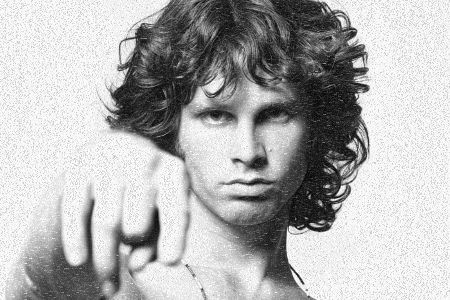
\includegraphics[scale=0.5]{./3sombras/Jim3.png}
  }
  \subfigure[Roberto3.bmp] {
    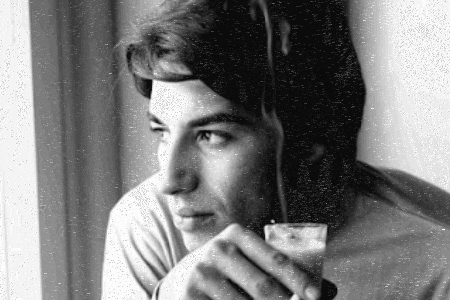
\includegraphics[scale=0.5]{./3sombras/Roberto3.png}
  }
  \subfigure[Whitney3.bmp] {
    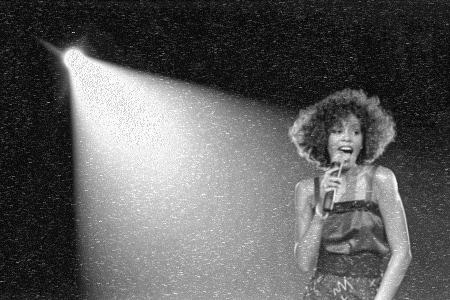
\includegraphics[scale=0.5]{./3sombras/Whitney3.png}
  }
  \subfigure[Shakira3.bmp] {
    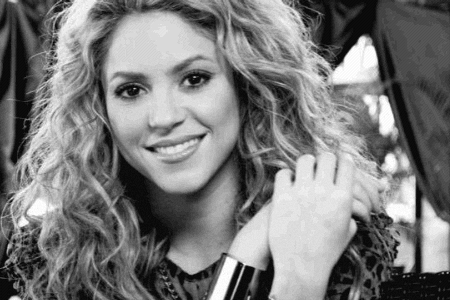
\includegraphics[scale=0.5]{./3sombras/Shakira3.png}
  }
   \subfigure[Recuperación obtenida] {
    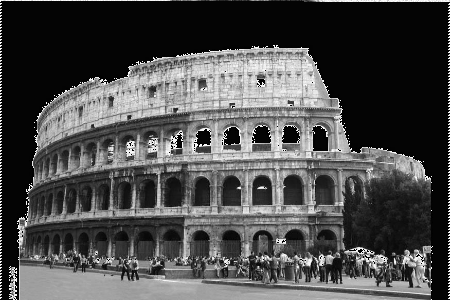
\includegraphics[scale=0.5]{./3sombras/resultado.png}
  }
   \caption{Recuperación con 3 sombras}
  \label{fig:3sombras}
\end{figure}

\begin{figure}[h!]
  \subfigure[Carlitos2.bmp] {
    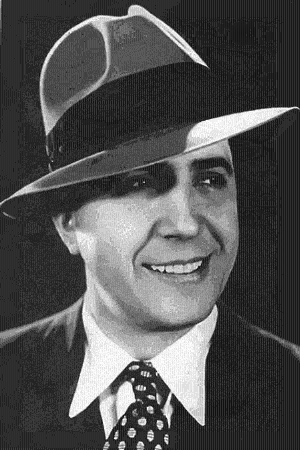
\includegraphics[scale=0.4]{./2sombras/Carlitos2.png}
  }
  \subfigure[Gandhi2.bmp] {
    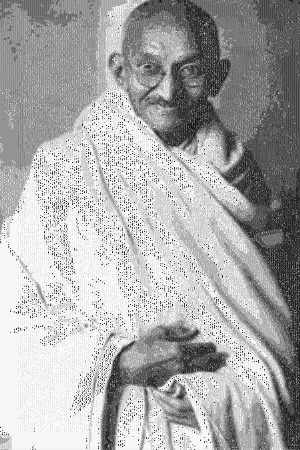
\includegraphics[scale=0.4]{./2sombras/Gandhi2.png}
  }
  \subfigure[Gandhi2.bmp] {
    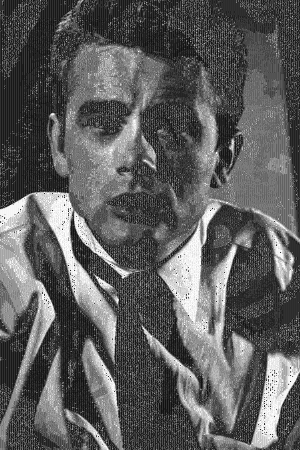
\includegraphics[scale=0.4]{./2sombras/James2.png}
  }
  \subfigure[Recuperación obtenida] {
    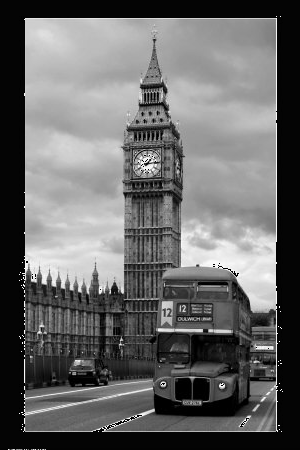
\includegraphics[scale=0.4]{./2sombras/resultado.png}
  }
  \caption{Recuperación con 2 sombras}
  \label{fig:2sombras}
\end{figure}

\begin{figure}[h!]
  \subfigure[James4.bmp] {
    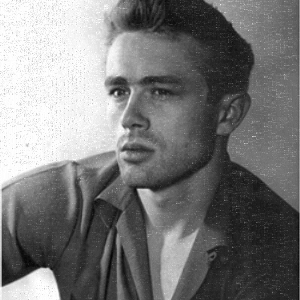
\includegraphics[scale=0.5]{./4sombras/James4.png}
  }
  \subfigure[Eva4.bmp] {
    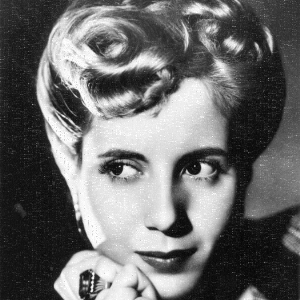
\includegraphics[scale=0.5]{./4sombras/Eva4.png}
  }
  \subfigure[Albert4.bmp] {
    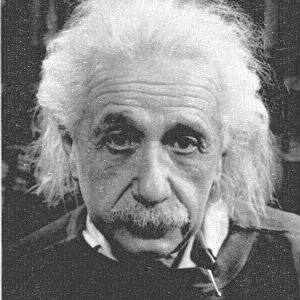
\includegraphics[scale=0.5]{./4sombras/Albert4.png}
  }
  \subfigure[Gustavo4.bmp] {
    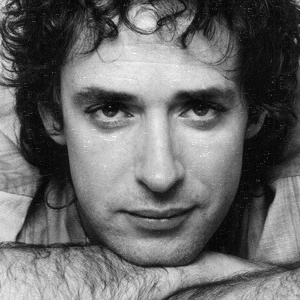
\includegraphics[scale=0.5]{./4sombras/Gustavo4.png}
  }
  \subfigure[Marilyn4.bmp] {
    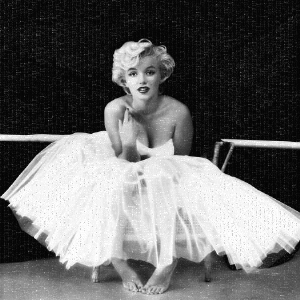
\includegraphics[scale=0.5]{./4sombras/Marilyn4.png}
  }
   \subfigure[Recuperación obtenida] {
    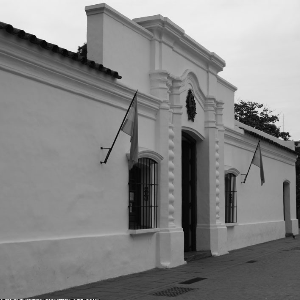
\includegraphics[scale=0.5]{./4sombras/resultado.png}
  }
   \caption{Recuperación con 4 sombras}
  \label{fig:4sombras}
\end{figure}


\end{document}